%%%%%%%%%%%%%%%%%%%%%%%%%%%%%%%%%%%%
% This is the template for submission to MICRO 2015
% The cls file is a modified from  'sig-alternate.cls'
%%%%%%%%%%%%%%%%%%%%%%%%%%%%%%%%%%%%

\documentclass{sig-alternate}

\newcommand{\ignore}[1]{}
\usepackage{fancyhdr}
\usepackage[normalem]{ulem}
\usepackage[hyphens]{url}
\usepackage{hyperref}
\usepackage{color}
\usepackage{booktabs}

%%%%%%%%%%%---SETME-----%%%%%%%%%%%%%
\newcommand{\microsubmissionnumber}{XXX}
%%%%%%%%%%%%%%%%%%%%%%%%%%%%%%%%%%%%

\fancypagestyle{firstpage}{
  \fancyhf{}
\setlength{\headheight}{50pt}
\renewcommand{\headrulewidth}{0pt}
%  \fancyhead[C]{\normalsize{\textbf{Columbia University Technical Report} \\ Department of Computer Science \\ CUCS-00117/April 18,2017\\ Van Bui and Martha A. Kim}}
%      \textbf{\#} -- Confidential Draft}} 
  \pagenumbering{arabic}
}  

%%%%%%%%%%%---SETME-----%%%%%%%%%%%%%
\title{Analysis of Super Fine-Grained Program Phases \\ \vspace{0.7cm} \large{\textbf{Van Bui and Martha A. Kim}} \\  \vspace{0.2cm} \normalsize{Columbia University Technical Report \\ Department of Computer Science \\ TR No. CUCS-001-17 \\ April 18,2017}} 
%%%%%%%%%%%%%%%%%%%%%%%%%%%%%%%%%%%%

\begin{document}
\maketitle
\thispagestyle{firstpage}
\pagestyle{plain}
\newcommand{\fixme}[1]{\textcolor{red}{#1}}


%%%%%% -- PAPER CONTENT STARTS-- %%%%%%%%

\sloppy
\begin{abstract}
Dynamic reconfiguration systems guided by coarse-grained program phases has found success in improving overall program performance and energy efficiency. These performance/energy savings are limited by the granularity that program phases are detected since phases that occur at a finer granularity goes undetected and reconfiguration opportunities are missed.  In this study, we detect program phases using interval sizes on the order of tens, hundreds, and thousands of program cycles. This is in stark contrast with prior phase detection studies where the interval size is on the order of several thousands to millions of cycles.  The primary goal of this study is to begin to fill a gap in the literature on phase detection by characterizing super fine-grained program phases and demonstrating an application where detection of these relatively short-lived phases can be instrumental. Traditional models for phase detection including basic block vectors and working set signatures are used to detect super fine-grained phases as well as a less traditional model based on microprocessor activity. Finally, we show an analytical case study where super fine-grained phases are applied to voltage and frequency scaling optimizations. 
\end{abstract}


\section{Introduction}

Program phase analysis has a history dating back to the 1960s where the notion of a working set (recently referenced objects) was introduced and applied to multi-programmed memory management~\cite{Glaser:1965:SDC}. Since that time, phase analysis has been applied to an extensive application space. A common application of phase analysis is guiding dynamic hardware reconfiguration policies. Some examples include configurable caches/tlbs~\cite{903259}\cite{Veidenbaum:1999:ACL}\cite{Albonesi:1999:SCW}, allocation of memory hierarchy resources~\cite{Balasubramonian:2000:MHR}\cite{Ranganathan:2000:RCA}, allocation of memory buffer resources~\cite{Veidenbaum:1999:ACL}, configurable branch predictors~\cite{694771}, configurable instruction windows~\cite{Buyuktosunoglu:2000:AIQ}\cite{Folegnani00reducingpower}, and configurable pipelines~\cite{Bahar:2001:PER}.  Other applications of phase analysis includes power reduction~\cite{Huang:2003:PAP}\cite{Isci:2006:PCP}, data cache prefetching~\cite{Lu:2003:PRD}, accelerating architecture simulations~\cite{Sherwood:2002:ACL}\cite{Perelman:2003:PSV}\cite{Lau:2006:SSP}\cite{Perelman:2006:DPP}, data race detection~\cite{Marino:2009:LES}, and invoking garbage collection~\cite{Xian:2007:MAP}. This very rich application space underscores the need for continued research in phase analysis to improve upon existing state-of-the-art phase detection techniques.

Prior research on program phase detection has studied the problem at a relatively coarse level of granularity, detecting phases at a resolution of several thousands to millions of program cycles~\cite{Lau:2005:MVL}\cite{Huffmire:2006:WPC}\cite{Isci:2006:PCP}.  This is partly because phase detection mechanisms account for operating system context switch overheads that can be on the order of millions of cycles. The phases that are analyzed in the current study are much more fine-grained patterns of program behavior that occur over intervals that are much shorter than millions of program cycles. These shorter phases should be applied to situations where associated overheads are much shorter then overheads usually incurred by the operating system (e.g. dynamic hardware reconfiguration). 

Prior studies suggests that fine-grained phase analysis incurs high overheads while providing modest returns~\cite{Magklis:2003:PDV}\cite{Huang:2003:PAP}. We contend that phase detection overheads can be mitigated by more efficient hardware designs. Continued efforts to reduce overheads due to resource reconfiguration also cut into the overall costs. As a noted example, research has shown that DVS  can incur overheads on the order of just tens of nanoseconds (rather then microseconds) now with the help of on-chip switching regulators~\cite{Kim:2011:FLD}\cite{Kim:2008:HPC}. The underlying question, which is outside the scope of this study, is what overhead levels can be tolerated by super fine-grained (SFG) phase analysis. The focus of the present study is to characterize these SFG phases and to begin to investigate promising application spaces. 

The task of detecting SFG phases can be considered within the much broader context of the phase shift detection (PSD) problem. The PSD problem takes as input a profile that encodes the time varying execution behavior of a program (along with a set of inputs stipulating how phases will be detected) and outputs a partitioning of the profile into periods of phases and phase transitions. Phases indicate periods of execution with similar behavior. The PSD problem input parameters are set by the client. The client can be any entity that utilizes the output of the PSD problem towards some purpose. The client has a producer-consumer like relationship within the PSD framework. We are interested in an instance of the PSD problem that will generate SFG phases, which are phases that will last for just tens or up to a few million of program cycles.

The input parameters to the PSD problem specifying how phases will be detected have previously been classified into two categories: \emph{granularity} and \emph{similarity}~\cite{Hind03phaseshift}. The granularity precisely defines the characteristics of the units that are compared for similarity. The similarity parameter defines a boolean function that computes whether two strings are similar or not based on a given threshold. The current study evaluates the SFG phases that emerge with relatively short interval size (granularity parameter) while also varying other similarity parameters. 

These are the overall goals of this research: 

\begin{enumerate}
\item Characterize SFG phases based on traditional and non-traditional models.
\item Compare and contrast phases that emerge as parameters such as interval size and similarity thresholds change.
\item Specify application spaces that can benefit from using SFG phases.
\end{enumerate}




\section{Related Work}

\subsection{Conventional Phase Analysis Techniques}
Program phase detection can be divided into techniques that define phases based on control flow, program counter, or performance characteristics. Each of these phase detection techniques define a model of program behavior over each interval based on some program characteristic.

For program counter and performance characteristics based approaches, usually a fixed length interval is defined or the interval can vary in size. Working set signatures~\cite{Dhodapkar:2002:MMH} is an example of a program counter based approach. The premise behind working set signatures is that program phases are a function of the set of executing instructions. The working set signature is an encoding of the executed instructions over an interval.  For performance characteristics based approaches to phase classification, a common performance metric used is IPC; several other metrics have been used including cache miss rate, TLB miss rates, and even power consumption~\cite{Balasubramonian:2000:MHR}\cite{Isci:2006:PCP}. 

Control flow based techniques characterize intervals based on the control-flow behavior of a program (e.g. functions, loops, and branches)~\cite{Huang:2003:PAP}\cite{Shen:2004:LPP}\cite{Zhang:2015:MPA}. Basic block vector (BBV)~\cite{Sherwood:2002:ACL} is an example of a control flow based approach. A basic block vector represents the set of basic blocks that execute over an interval. The idea behind basic block vectors is that program behavior can be modeled as a series of code blocks.

\subsection{Hierarchical Phase Analysis}

A phase hierarchy consists of longer duration phases composed of shorter running phases. Zhang et al~\cite{Zhang:2015:MPA} observed that coarse-grained intervals that belong to the same phase actually consists of stably distributed fine-grained phases. Phase hierarchies have been visualized using various techniques (e.g. multi-dimensional accumulated respresentation) to demonstrate their existence~\cite{Lau:2005:MVL}. Phase hierarchies imply that phases can form at different levels of granularity from very coarse to very fine-grained.

Shen et al~\cite{Shen:2004:LPP} identifies locality phases, which characterizes program memory behavior based on data reuse distances. A combination of wavelet filtering and grammar compression is applied to identify locality phases. 

Lau et al~\cite{Lau:2005:MVL} identify program phases using a performance metric (CPI) and k-means clustering to cluster together similar intervals at different levels of a variable length interval hierarchy. They use the Sequitur algorithm to determine the variable length intervals. They show in the paper that hierarchical phase behavior exists using visualization techniques known as 2D accumulated representation and 3D non-accumulated representation. In 3D non-accumulated representation, each point in the three dimensional space is a BBV (reduced down to three dimensions) and each edge is simply BBVs that are adjacent to each other in time. In 2D accumulated representation, the number of times each basic block is executed in an interval is also being encoded and the space is reduced down to two dimensions for visualization purposes. 


\section{Interval Models}

An interval is modeled in such a way that enables a quantitative comparison of intervals to one another for similarity. The models that we use to detect SFG phases includes the instruction working set, basic block vectors, and Intel Top-Down. 

\subsection{Instruction Working Set Signature}

An instruction working set (IWS)~\cite{Dhodapkar:2002:MMH} is the set of instructions touched over a fixed interval of time. The relative working set distance between intervals $i$ and $i-1$ is defined as 

\begin{center}
$\delta_{i,i-1} = \frac{||W_i \bigcup W_{i-1}||-||W_i \bigcap W_{i-1}||}{||W_i \bigcup W_{i-1}||}$
\end{center}
where $W_i$ is the working set for interval $i$.
 
A working set signature is a lossy-compressed representation of a working set. The program counter is sampled over a fixed interval of instructions. A hashing function is applied to the sample to set a bit in an $n$-bit vector, which represents the signature (See Figure~\ref{fig:signature}). Phase changes are detected by computing the relative signature distance between intervals and comparing the distance against some pre-determined threshold. The hardware complexity of this technique is dependent on the working set size.

\begin{figure}[htbp]
  \begin{center}
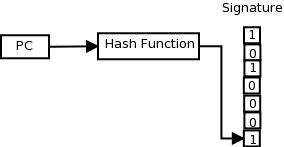
\includegraphics[width=0.60\columnwidth]{figs/workingsetsignature}
  \end{center}
  \caption{Generating the working set signature.}
  \label{fig:signature}
\end{figure}

\subsection{Basic Block Vectors}

Basic block vectors (BBV)~\cite{Sherwood:2003:DEP} encodes the execution frequency of basic blocks over an interval. BBVs can be approximated using an array of accumulators (counters) that tracks the number of instructions executed by a basic block in a given execution interval (see Figure~\ref{fig:bbv}). When a branch PC is encountered, a hash function is applied to the PC to determine an index into the accumulator table in order to increment the appropriate counter by the number of committed instructions since the last branch instruction. The BBV difference between intervals is computed using the manhattan distance. A phase change is determined by comparing the BBV difference to a difference threshold. The hardware required to implement BBVs includes an N-bit wide RAM array for the accumulator table, sampling hardware to detect branch instructions and analyze the retire stream, and an N-bit adder to update the accumulator table. The hardware complexity of BBV is much higher compared to working set signatures. 

\begin{figure}[htbp]
  \begin{center}
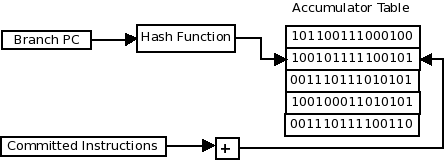
\includegraphics[width=0.80\columnwidth]{figs/bbv}
  \end{center}
  \caption{BBV accumulator table update technique.}
  \label{fig:bbv}
\end{figure}

\subsection{Intel Top-Down Classification}
\label{sec:topdown}

Intel Top-Down (ITD)~\cite{Yasin:2014:TDM} classifies pipeline activity very broadly into four categories: \textbf{frontend bound}, \textbf{bad speculation}, \textbf{retiring}, and \textbf{backend bound} (see Figure~\ref{fig:topdown2}). Each of these categories can be broken down even further and differently depending on the architecture. Below we describe the four top-level categories for the LEON3 (32-bit SPARC V8 architecture) instruction pipeline since this is the architecture used in our measurements.

\textbf{Frontend Bound.} The frontend includes the front portion of the pipeline where the branch predictor predicts the next address, instructions are fetched and decoded, and the register file is accessed. The frontend prepares instructions to be executed by the backend of the processor. Cycles are classified as frontend bound when the frontend undersupplies the backend of the pipeline (e.g. instruction cache misses).

\textbf{Bad speculation.} This category captures inefficiency in the pipeline due to incorrect speculation by the branch predictor. This includes issued instructions that do not eventually get retired. These instructions are annulled (i.e. has no effect and effectively not executed) in the LEON3.  

\textbf{Retiring.} This category is for issued instructions that eventually get retired. 

\textbf{Backend Bound.} A cycle is classified as backend bound when a new instruction is not issued to the execution unit in a given cycle while the frontend of the pipeline is not stalled. This may be due to data cache misses or overloaded functional units. The backend category can be further broken down into \emph{core bound} and \emph{memory bound}. 

\begin{itemize}
\item [--] \underline{Core bound} includes stalls due to overloaded functional units.
\item [--] \underline{Memory bound} includes store bound (i.e. high number of buffered stores), L1 bound (cache access), and memory bound (cache miss).
\end{itemize}

\begin{figure}[htbp]
  \begin{center}
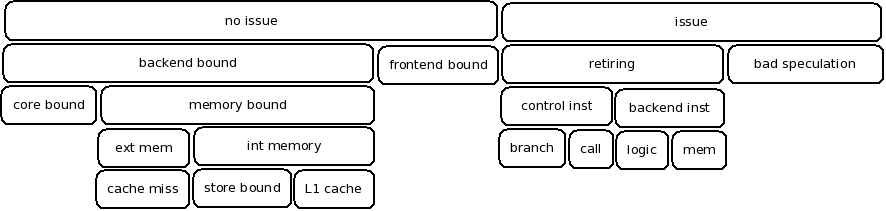
\includegraphics[width=0.99\columnwidth]{figs/topdown2}
  \end{center}
  \caption{An example of the Intel Top-Down processor activity categories.}
  \label{fig:topdown2}
\end{figure}

Traditionally, the ITD categories has been used for the purpose of detecting sources of performance bottlenecks. The motivation for using the ITD classification to detect SFG phases is that the different categories provides different levels of detail regarding pipeline activity, which we think is a good model for program behavior. Furthermore, hardware complexity is significantly reduced since only a finite vector of size $n$ is necessary to store the frequency of each category over an interval, where $n$ is the number of categories at each level. By comparison, the hardware complexity is a function of the number of unique instructions in the case of IWS and the number of unique basic blocks in the case of BBVs, which can be difficult to determine a priori. The ITD vector difference between intervals is computed using the Manhattan distance, similar to the BBV difference.





\section{Methodology}

We collected entire program profiles for nine different benchmarks. Eight of the benchmarks came from the MiBench~\cite{Guthaus:2001:MFC} benchmark suite, which covered applications in auto, office, network, security and telecommunication. The MiBench benchmarks measured includes \emph{basicmath, bitcount, qsort, stringsearch, dijkstra, sha, fft,} and \emph{ifft}. We made modifications to the input and output functionality to these benchmarks in order to run them as baremetal applications on an FPGA board. We also added matrix multiply (10x10 matrices) since it is a common kernel for several applications. We ran the MiBench benchmarks using the small input data set, which was of sufficient length to allow us to collect profiles in a reasonable amount of time while also long enough for detecting SFG phases, which was our primary goal.

All the benchmarks were run on a 32-bit LEON3 processor, which is based on the SPARC V8 RISC architecture. A LEON3 Verilog/VHDL customized core design was synthesized and ran on a Xilinx VC707 FPGA board. We added additional logic to the design in order to support tracing various core processor signals. The signals collected included the program counter, instruction type, processor stalls, bus activity, register file activity, and various other signals along the integer pipeline necessary for building the models and for analysis off-line. The signals were packed into 32-bits and stored in SRAMS ($\approx$4MB). When the SRAMS were filled up during runtime, an interrupt is generated and an interrupt handler reads and stores the samples to main memory. We looked at the overheads generated from the measurements and found that the highest overhead observed is 0.03\% for \textbf{basicmath}, which we believe to be reasonable. 

The PSD input parameters that are varied in our analysis includes the interval size, similarity threshold, and interval models. The minimum size of a phase is defined to be two intervals long here. The range for the interval size is 1-100K (cycles) and the similarity threshold range is between 0 and 1, where 0 indicates perfect similarity and 1 indicates not similar. The intervals are modeled as instruction working sets, basic block vectors, CPI, and also using the Intel Top-Down classification. The CPI is included as a reference point to assess how phases generated using IWS, BBV, and ITD compare to a purely performance driven model. We also only present averages across benchmarks here since we are primarily interested in analyzing the high-level trends in phase behavior that emerge as we vary these input parameters.


\section{Phase Characterization}

Phases can be characterized in many ways (e.g. phase duration, performance, power utilization, etc). For the SFG phases that we are studying, we look at the phase length, phase transitions, and phase coverage. The phase length is an important characteristic to consider because it guides the client's decision to apply an optimization that makes sense given the amount of time the phase will last for. Ideally, the phase will last long enough to amortize the cost for applying the new configuration. The phase transitions is important to consider since it may factor into the explore time overhead, which is the period when the client recognizes a phase shift and explores different configurations. Consecutive phase transitions that result in the same configuration by the client wastes the time and resources in exploring. A lower number of phase transitions is ideal along with only phase transitions that are significant enough to require a new configuration. The phase coverage is the percentage of the application that has been classified as in-phase as opposed to in transition. The higher the phase coverage, the more impact an optimization applied by the client can have on the code as a whole. While there are several other phase characteristics, we select to study phase length, phase transition, and phase coverage since they are critical characteristics that commonly factor into a cost-benefit analysis made by the client.       

\subsection{Phase Length}
Here, we analyze how the phase length changes as parameters such as the model, interval size, and similarity threshold varies. The \emph{low} threshold value ($t$) is set to $t=0.1$ and the \emph{high} threshold value is set to $t=0.9$. When otherwise not noted, $t=0.1$. The computed similarity values $s$ has range $0 \leq s \leq 1.0$, where $0$ indicates intervals that are perfectly similar and $1$ indicates intervals that are not at all similar. If a computed similarity value falls below the threshold, then the tested intervals are considered similar enough to form a phase. The interval size $i$ we allow to vary between 1 and 100K. The evaluated models include instruction working sets (IWS), basic block vectors (BBV), Intel Top Down (ITD), and CPI. 

\begin{figure}[htbp]
  \begin{center}
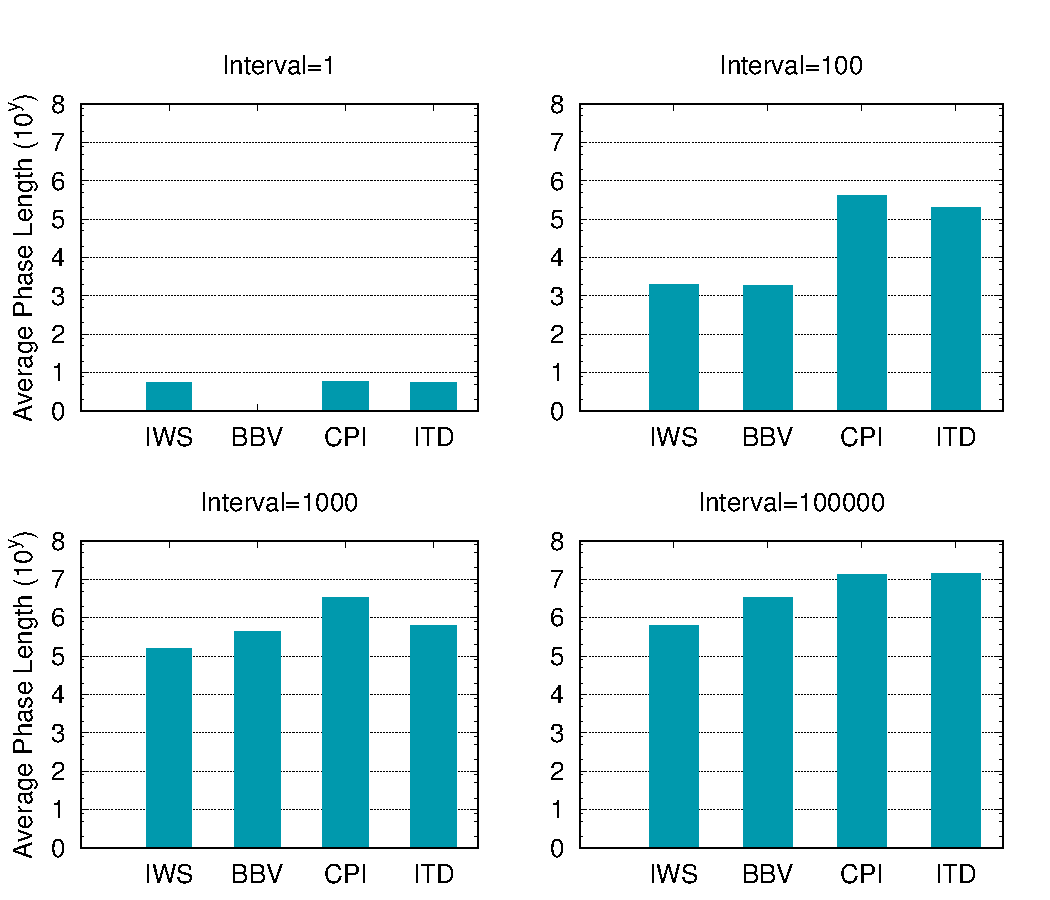
\includegraphics[width=0.99\columnwidth]{figs/phaselenavg}
  \end{center}
  \caption{At very short intervals, the phase lengths are similar across models. At longer intervals, differences in phase length begins to emerge between models.}
  \label{fig:phaselenavg}
\end{figure}

Figure~\ref{fig:phaselenavg} shows the absolute average phase length across different models and interval sizes. The range in phase length that can be observed is roughly 5-10M cycles long. The phases detected on the lower end of the size spectrum would be undetectable had the interval size been restricted to be much higher (e.g. 1M cycles). Another key observation is that the model deployed along with the interval size can have a significant effect on the phase length.  At an interval size of one cycle, we see little differences in the average phase length, which turns out to be roughly five cycles across models. As the interval size increases, we begin to see more separation with respect to the phase length across models. At an interval size of 100, both CPI and ITD have average phase lengths a couple of orders of magnitude higher then IWS and BBV. At even higher interval sizes, up to 100K, we still see some differences between models (about one order of magnitude difference). The interval size and model should be appropriately configured by the client to produce the desired phase length.

Figure~\ref{fig:phaselen} shows how the average phase length changes across the nine benchmarks as we vary all three parameters (interval size, model, and similarity threshold). One clear trend is that the phase length tends to grow as the interval size is increased. The growth rate is fast at smaller interval sizes and slows down at larger interval sizes. With respect to the similarity threshold, we see a much more pronouced growth in phase length at smaller interval sizes for higher threshold values. Along the same vein, we also generally see a much more pronounced slowdown of the growth in phase length at a higher threshold and interval size. Also note from Figure~\ref{fig:phaselen} the difference in phase length across the models. ITD tends to track more closely to CPI while IWS and BBV is tracking more closely with respect to phase length. Another interesting observation is that both CPI and ITD tend to have longer phase lengths with the former having the longest phase length, but this gap narrows given a higher threshold and interval size. To summarize, we observe the following trends with respect to phase length:

\begin{enumerate}
\item The phase length increases as the interval size increases.
\item The phase length increases at a faster rate given a higher threshold.
\item ITD tends to have a longer phase length compared to IWS and BBV and tracks more closely to CPI.
\end{enumerate}

The phase length as previously mentioned is of interest to the client in order to perform a cost benefit analysis of applying a new configuration. As Figure~\ref{fig:phaselen} shows, all three parameters (interval size, model, and similarity threshold) can impact the phase length and can be tweaked by the client in order to obtain the desired length. If a client desires a longer phase length, then that can be accomplished by increasing the interval size, relaxing the threshold, or switching models. The design of a phase analysis framework should enable the client to easily adjust these parameters to achieve the desired phase length. 


\begin{figure}[htbp]
  \begin{center}
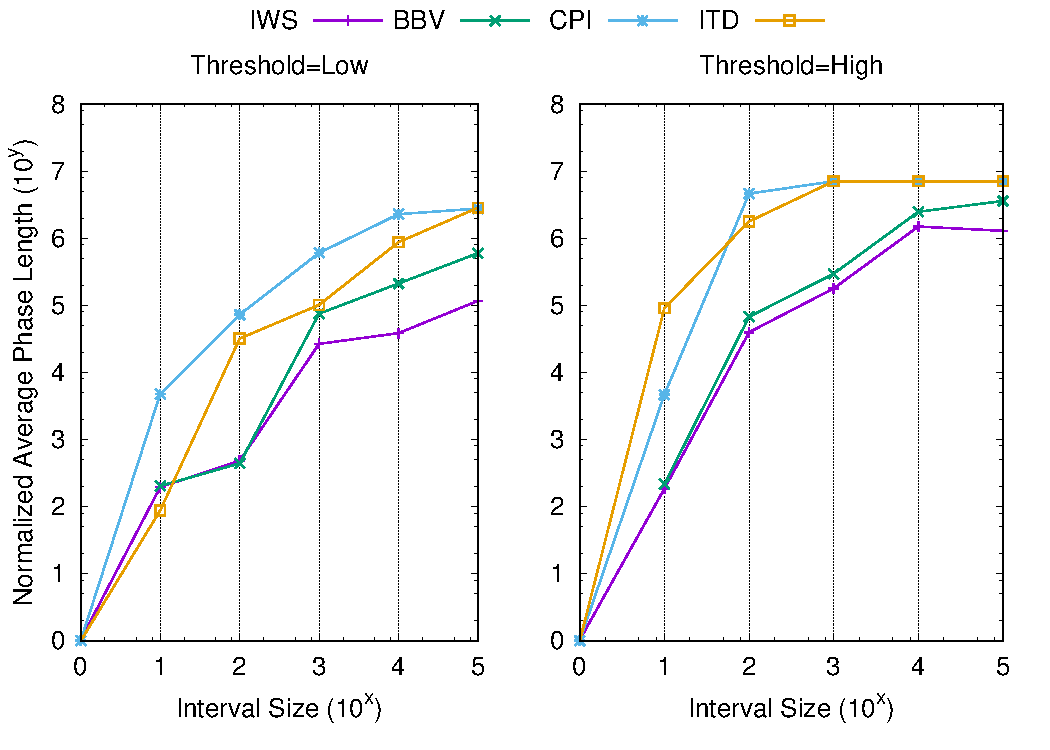
\includegraphics[width=0.99\columnwidth]{figs/phaselenfixthreshold}
  \end{center}
  \caption{All three parameters (interval size, model, and threshold) appear to have a significant effect on the phase length.}
  \label{fig:phaselen}
\end{figure}




\subsection{Phase Transitions}
Similar to the phase length analysis, we also vary the interval size, model, and similarity threshold and evaluate changes in phase transitions. As Figure~\ref{fig:phasetransavg} shows, as the interval size increases, the number of phase transitions tend to decrease. At higher thresholds, we see a separation in phase transition between IWS/BBV and ITD/CPI. Recall that in the phase length analysis, ITD tracked pretty closely with CPI as well and IWS and BBV tracked closely with each other. There appears to be a stabilization in the number of phase transitions at an interval size of 100 for the high threshold case for ITD and CPI, which coincides with the point at which the phase length for ITD and CPI begins to stabilize with increasing interval size as shown in Figure~\ref{fig:phaselen}. This suggests that increasing the interval size has the joint effect of increasing the phase length and decreasing the number of phase transitions, but that there does exist a stabilization point for which there will be little change in phase length and phase transitions. At low thresholds, we see very similar behavior in phase transition across models. In general, if a reconfiguration client is interested in lowering exploration costs by decreasing the number of phase transitions, it appears that the best avenue is to increase the interval size, but to also recognize there exists a limit as the number of phase transitions reaches it's minimum value and phase length reaches it's maximum value (i.e. a phase can not last longer then the duration of the program).  At higher thresholds, this stabilization in phase transitions and phase length occurs at a much earlier point as the interval size increases. 

\begin{figure}[htbp]
  \begin{center}
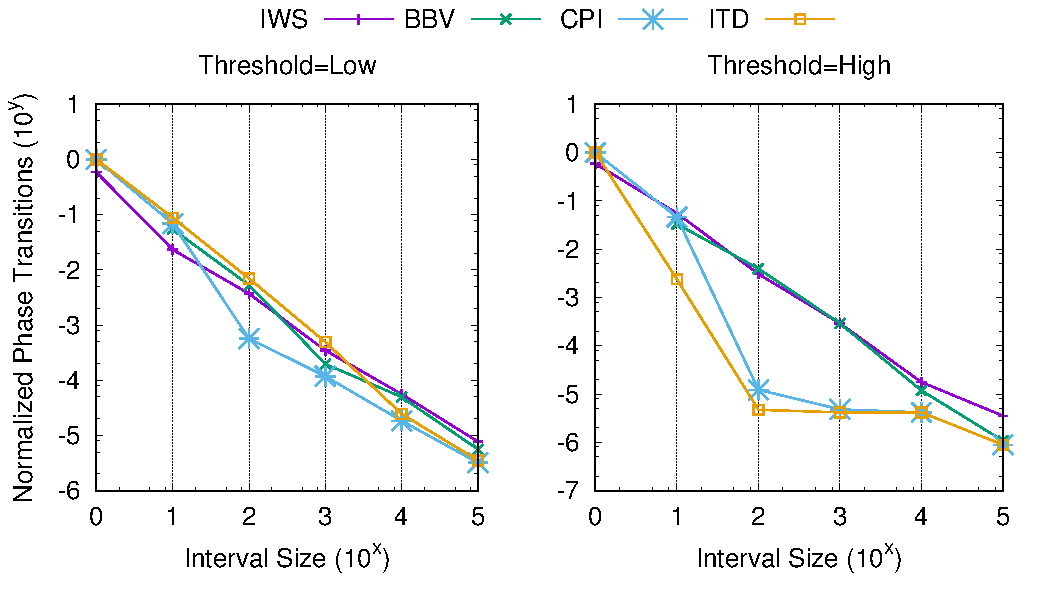
\includegraphics[width=0.95\columnwidth]{figs/phasetransavg}
  \end{center}
  \caption{The interval size is the most effective parameter for varying the phase transition compared with the model and threshold. But the threshold value does impact the rate at which the phase transitions decrease as the interval size grows and this behavior appears to vary between models.}
  \label{fig:phasetransavg}
\end{figure}





\subsection{Phase Coverage}
The phase coverage determines the proportion of the program where phase behavior has been defined. Periods of execution where phase behavior has not been defined is considered to be phase transition periods. The phase coverage determines the percentage of the application that can benefit from some client-side optimization and so ideally a high level of phase coverage is preferable. 

Figure~\ref{fig:phasecycles} shows that the phase coverage is not very well behaved with respect to the interval size. That is, as the interval size increases, there is no clear trend in phase coverage. By contrast, there does appear to be some consistent trends for phase coverage with respect to the threshold and model. A higher threshold appears to increase the phase coverage. CPI followed closely by ITD also appears to have higher phase coverage compared to IWS and BBV, with IWS generally having the lowest phase coverage. As far as configuration clients are concerned, adjusting the model as well as increasing the similarity threshold should effectively increase the phase coverage.

\begin{figure}[htbp]
  \begin{center}
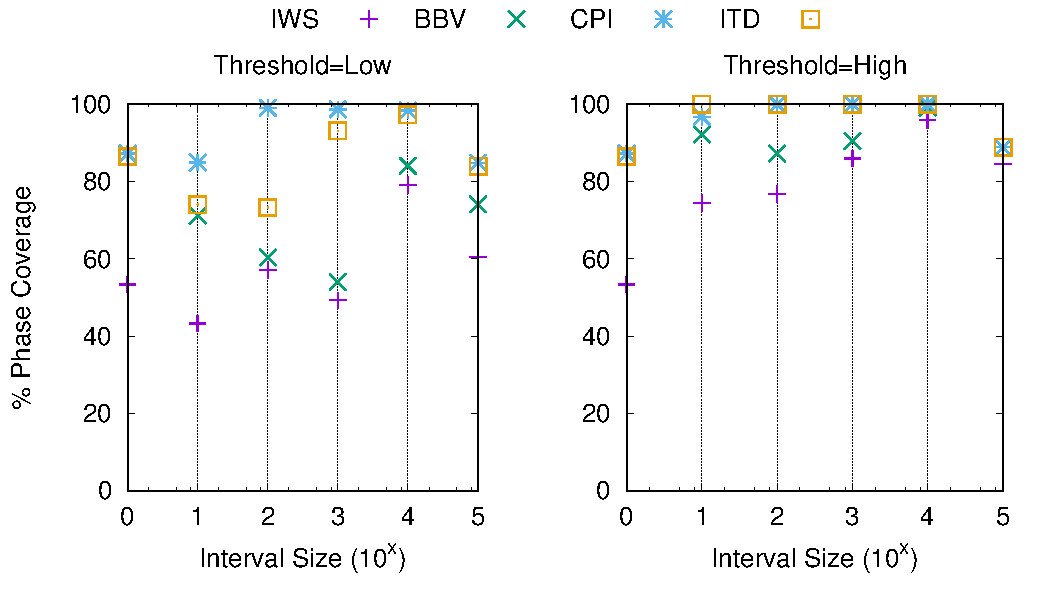
\includegraphics[width=0.99\columnwidth]{figs/phasecyclesthreshold}
  \end{center}
  \caption{Increasing the similarity threshold and using particular models (such as ITD) will tend to result in higher phase coverage.}
  \label{fig:phasecycles}
\end{figure}



\section{DVFS Application}

We have described the different characteristics of SFG phases and also show that these characteristics can be tweaked by adjusting certain parameters including the interval size, similarity threshold, as well as the model. A key question that has not been addressed yet is how these SFG phases can be exploited by the client. In this section, we explore how SFG phases can guide DVFS. 

The DVFS algorithm we deploy varies the voltage and frequency settings based on the CPI for a given phase. Table~\ref{tab:pstates} shows the mapping between CPI ranges and voltage/frequency states for the LEON3. The general idea is that when the CPI is high and processor is running less efficiently, both the voltage and frequency are scaled down in order to trade-off lower power for a small penalty in performance. This trade-off in performance and power is what we call here the performance degradation to power savings ratio. During periods of phase transition, the processor is assumed to be running in Turbo mode. 

\begin{table}[ht]
\caption{LEON3 Prototype P-States}
\label{tab:pstates}
\centering
\begin{tabular}{|l|c|c|c|}
\hline
\textbf{Name} & \textbf{CPI} &  \textbf{Voltage (V)} & \textbf{Freq (MHz)}   \\ \hline \hline
 Turbo & $< 1.5$ & 1.00 & 1000  \\ \hline
 Eff1 & [1.5,2.0) & 0.85 & 700  \\ \hline
 Eff2 & [2.0,2.5) & 0.75 & 550   \\ \hline
 Eff3 & $\geq 2.5$ & 0.60 & 320   \\ \hline
\end{tabular}
\end{table}

The parameters used in the performance and power models for our analysis are specific to our own design of the LEON3 processor. The total time is computed as the sum of time spent at each P-state.

\begin{center}
$T_{total} = \sum\limits_{i=1}^P \frac{N_i}{F_i}$
\end{center}

where $P$ is the number of P-states, $N_i$ is the total cycles spent in P-state $i$, and $F_i$ is the clock frequency in P-state $i$ (noted in Table~\ref{tab:pstates}). 

Total power is computed as follows:

\begin{center}
$P_{total} = \frac{\sum\limits_{i=1}^P (\alpha CV_i^2F_i +V_iI) \times T_i}{T_{total}}$
\end{center}

where $\alpha$ is the activity factor, $C$ is the switching load capacitance,  $V_i$ is the voltage in P-state $i$, $I$ is the leakage, and $T_i$ is total time spent in P-state $i$. In order to estimate the activity and capacitance, we measured the dynamic power by back-annotation from simulation of the synthesized RTL at each P-state while running floating point benchmarks. Based on the dynamic power numbers obtained, we determined $\alpha \times C\approx 1.6e^{-10}$. The leakage was estimated in a similar fashion by measuring the static power and we set  $I\approx 0.03$. 

The results from applying a simple DVFS algorithm to the SFG phases show that at an interval of size one (the smallest possible interval size), the voltage and frequency scaling is much more aggressive compared to intervals greater than one. As Figure~\ref{fig:ratiodvfs} shows, at an interval of size 1, the performance degradation to power savings ratio is between the computed ratios for \textbf{Eff2} and \textbf{Eff3} across the models (BBV is excluded because basic blocks are defined here at intervals larger than one). At interval sizes greater than 1, the ratio is between the ratios for \textbf{Eff1} and \textbf{Eff2}. This suggests that at shorter intervals (and therefore much shorter in duration SFG phases), the algorithm is more adept at detecting very fine-grained shifts in CPI and respond by operating at lower V/F levels.  

\begin{figure}[htbp]
  \begin{center}
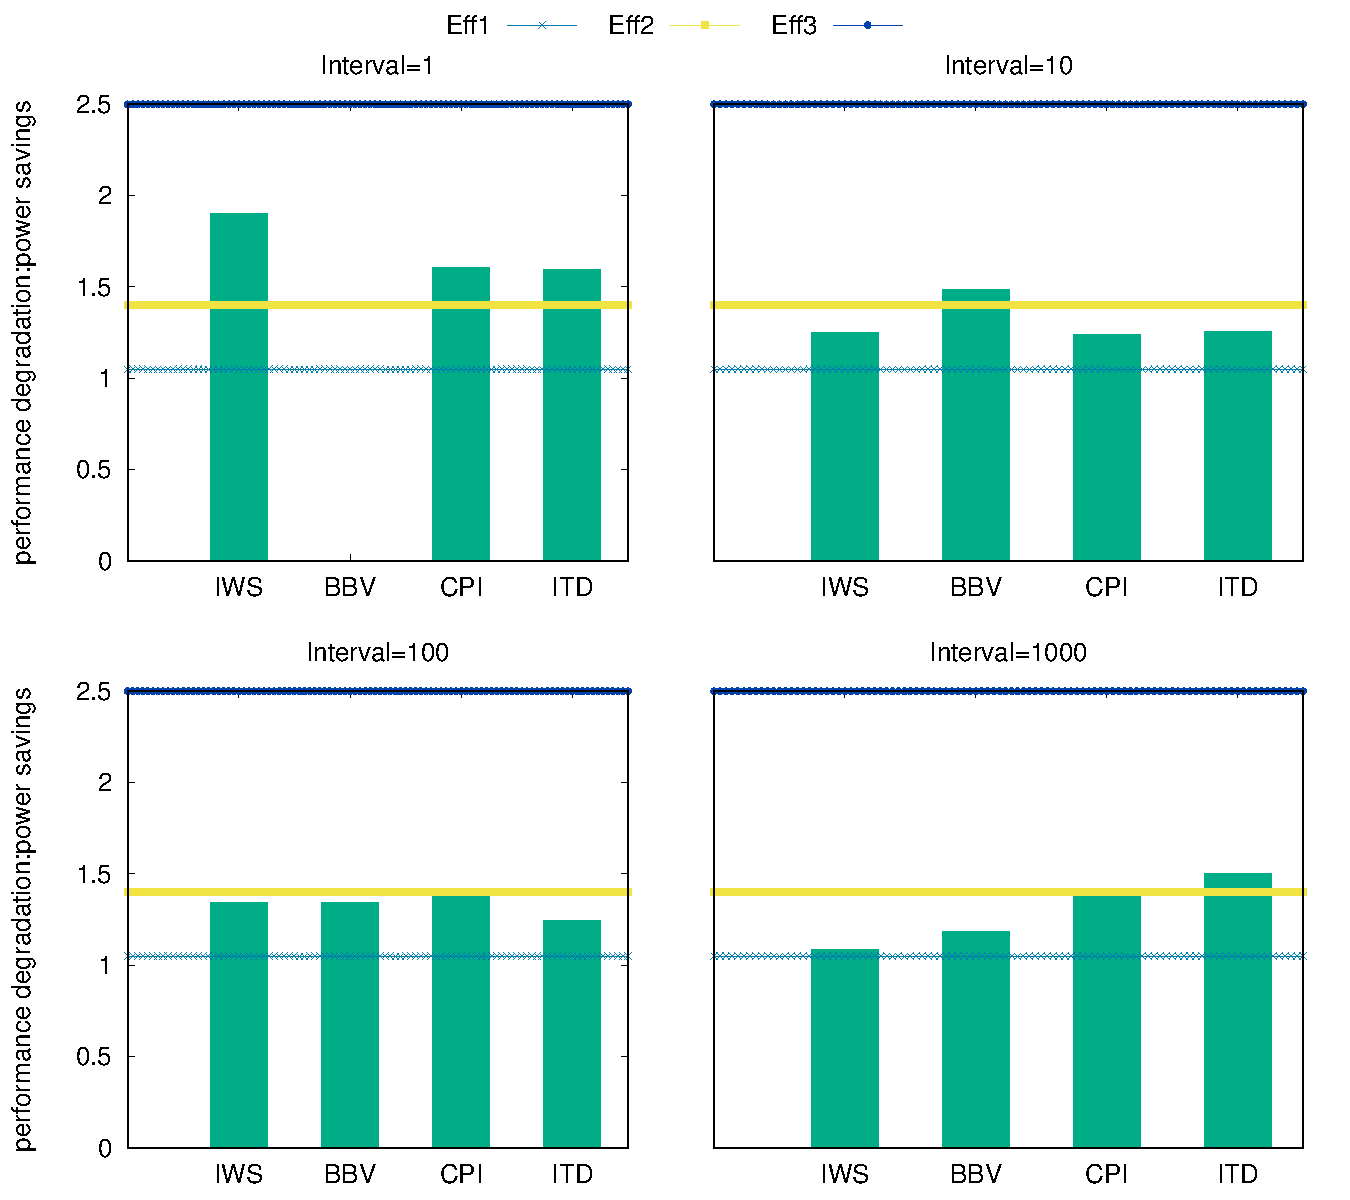
\includegraphics[width=0.99\columnwidth]{figs/ratiodvfs}
  \end{center}
  \caption{Shorter interval sizes result in much more aggressive voltage and frequency settings overall.} 

  \label{fig:ratiodvfs}
\end{figure}


\section{Conclusion}

This study has shown different characteristics of SFG phases and applied SFG phases to DVFS. Controls for various parameters such as the interval size, similarity threshold, and model impact the phase length, number of phase transitions as well as the phase coverage. The interval size significantly impacts the phase length and transition. The similarity threshold effects all three phase characteristics. Finally, the interval model effects phase length and coverage. Phase detection tools should allow the client maximum flexibility to tune these parameters to generate the phase characteristics that fit the best for their overall needs. 

As the DVFS study show, the interval size is a significant parameter to factor in as it results in very different performance degradation to power savings ratios at different interval sizes. Other clients may find useful configuration of a different set of parameters. In addition to DVFS, we think that other potential application areas to explore for SFG phases includes anomaly detection, clock gating, and performance monitoring. Based on the findings in the current study, we believe that these applications and possibly others can fully exploit SFG phases to generate dynamically secure, performance, and power efficient code executions.

\section*{Acknowledgment}                                                                                                                                                                                

The authors would like to thank Paolo Mantovani for providing the LEON3 code base and for the technical support and guidance provided throughout the project. In addition, we would like to thank the students and faculty from the computer architecture group at Columbia University for their feedback.                 

%%%%%%% -- PAPER CONTENT ENDS -- %%%%%%%%


%%%%%%%%% -- BIB STYLE AND FILE -- %%%%%%%%
\bibliographystyle{ieeetr}
\bibliography{ref}
%%%%%%%%%%%%%%%%%%%%%%%%%%%%%%%%%%%%

\end{document}
